\documentclass[11pt]{beamer}
\usetheme{Madrid}
\usepackage{amsmath,amssymb,amsfonts,graphicx}
\usepackage{multicol,multirow,booktabs}
\usepackage{tikz}
\usepackage{pgfplots}
\pgfplotsset{compat=1.17}
\usepackage{siunitx}
\sisetup{output-decimal-marker={.},separate-uncertainty=true}

% To fit long frames
\setbeamerfont{normal text}{size=\small}

\title{H2 Physics \\ Circular Motion}
\author{R.F.H.}
\date{\today}

\begin{document}

\begin{frame}
\titlepage
\end{frame}

% Section 1: Getting Prepared
\section{Getting Prepared}

\begin{frame}[shrink=15]{Brain Dump}
\centering
\Large
\textit{What do you know about Circular Motion?}
\vfill
\end{frame}

\begin{frame}[shrink=15]{Brain Dump (CONT'D)}
\centering
\Large
\textit{What do you know about Circular Motion?}
\vfill
\begin{itemize}
    \item Angular displacement $\theta$ (radians)
    \item Angular velocity $\omega = \frac{d\theta}{dt}$
    \item Relationship $v = r\omega$
    \item Centripetal acceleration $a_c = \frac{v^2}{r} = r\omega^2$
    \item Centripetal force $F_c = \frac{mv^2}{r} = mr\omega^2$
    \item Sources of centripetal force: tension, friction, gravity, normal force
    \item Applications: horizontal circles, vertical circles, banked curves, conical pendulum
    \item Non-uniform circular motion (tangential acceleration)
\end{itemize}
\end{frame}

\begin{frame}{Math Checklist}
Before tackling Circular Motion, ensure you are comfortable with:
\begin{columns}[T]
\column{0.5\textwidth}
\begin{itemize}
    \item Radians and degree-radian conversion
    \item Trigonometric functions ($\sin$, $\cos$, $\tan$)
    \item Solving equations with $\omega$, $T$, $f$
    \item Vector components
\end{itemize}
\column{0.5\textwidth}
\begin{itemize}
    \item Differentiation of $\sin$ and $\cos$ (for variable speed)
    \item Small angle approximations
    \item Quadratic equations
    \item Graphing sinusoidal functions
\end{itemize}
\end{columns}
\end{frame}

% Section 2: Concept Mastery
\section{Concept Mastery}

\begin{frame}{Building Intuition – Real-world Applications}
\begin{itemize}
    \item \alert{Car rounding a curve}: friction provides centripetal force; if too fast, skidding occurs.
    \item \alert{Amusement park rides}: loop-the-loop, rotor, gravitron – all rely on centripetal forces.
    \item \alert{Satellites in orbit}: gravity provides centripetal force; orbital speed determines radius.
    \item \alert{Centrifuge}: spinning rapidly to separate components based on density.
    \item \alert{Conical pendulum}: used in governors for engines.
    \item \alert{Banked roads}: design allows cars to turn at higher speeds without relying solely on friction.
\end{itemize}
\end{frame}

\begin{frame}{Formalization – Angular Quantities}
\begin{block}{Angular Displacement $\theta$}
Angle swept by the radius vector, measured in radians. $1\ \text{rad} = \frac{\text{arc length}}{\text{radius}}$.
\end{block}
\begin{block}{Angular Velocity $\omega$}
Rate of change of angular displacement: $\omega = \frac{d\theta}{dt}$. For uniform circular motion, $\omega = \frac{2\pi}{T} = 2\pi f$.
\end{block}
\begin{block}{Relation between Linear and Angular Quantities}
Arc length $s = r\theta$, speed $v = r\omega$, tangential acceleration $a_t = r\alpha$ (where $\alpha$ is angular acceleration).
\end{block}
\end{frame}

\begin{frame}[shrink=10]{Formalization – Centripetal Acceleration}
For an object moving in a circle of radius $r$ with constant speed $v$, the velocity vector changes direction continuously. The acceleration is directed toward the centre:
\[ a_c = \frac{v^2}{r} = r\omega^2 \]
\begin{center}
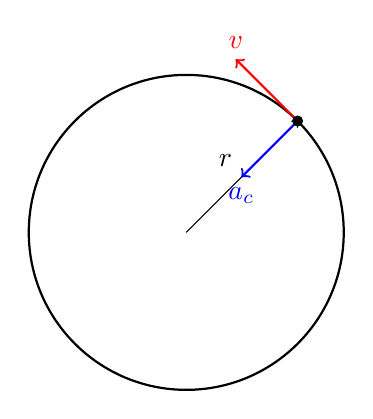
\begin{tikzpicture}
\draw[thick] (0,0) circle (2cm);
\draw[->] (0,0) -- (1.414,1.414) node[midway,above left] {$r$};
\draw[->,red,thick] (1.414,1.414) -- (0.628,2.2) node[above] {$v$};
\draw[->,blue,thick] (1.414,1.414) -- (0.7,0.7) node[below] {$a_c$};
\fill (1.414,1.414) circle (2pt);
\end{tikzpicture}
\end{center}
Derivation: Consider velocity vectors at two nearby points; the change $\Delta v$ points toward centre; $\frac{\Delta v}{v} \approx \frac{\Delta s}{r}$, so $a = \frac{\Delta v}{\Delta t} = \frac{v}{r}\frac{\Delta s}{\Delta t} = \frac{v^2}{r}$.
\end{frame}

\begin{frame}{Formalization – Centripetal Force}
By Newton's second law, a net force toward the centre is required:
\[ F_c = ma_c = \frac{mv^2}{r} = mr\omega^2 \]
This force is not a new type of force; it is provided by existing forces such as:
\begin{itemize}
    \item Tension (e.g., object on a string)
    \item Friction (e.g., car turning on flat road)
    \item Gravity (e.g., satellite in orbit)
    \item Normal force (e.g., banked curve, rotor ride)
    \item Combination of forces (e.g., vertical circle)
\end{itemize}
\end{frame}

\begin{frame}{Formalization – Vertical Circular Motion}
At different points, the centripetal force is provided by combinations of weight and tension/normal force.
\vspace{0.3cm}
\begin{columns}[T]
\column{0.5\textwidth}
\textbf{Top of circle:}
\[ T + mg = \frac{mv^2}{r} \]
Minimum speed to complete circle: when $T = 0$, $v_{\min} = \sqrt{gr}$.
\column{0.5\textwidth}
\textbf{Bottom of circle:}
\[ T - mg = \frac{mv^2}{r} \]
Tension is maximum here.
\end{columns}
\vspace{0.3cm}
Energy conservation often used to relate speeds at different points.
\end{frame}

\begin{frame}{Formalization – Banked Curves}
For a frictionless banked curve with angle $\theta$, the horizontal component of normal force provides centripetal force:
\[ N\sin\theta = \frac{mv^2}{r}, \quad N\cos\theta = mg \]
Dividing: $\tan\theta = \frac{v^2}{rg}$.
For a given $\theta$, there is one design speed. At other speeds, friction is needed.
\end{frame}

\begin{frame}{Micro-Testing – Quick Checks}
\begin{enumerate}
    \item A car rounds a flat curve at $20\ \mathrm{m/s}$. If the radius is $100\ \mathrm{m}$, what is the centripetal acceleration? \pause \alert{$a = v^2/r = 400/100 = 4\ \mathrm{m/s^2}$}.
    \item An object on a string in horizontal circular motion has constant speed. Is there work done on it? \pause \alert{No, because force is perpendicular to displacement.}
    \item What provides the centripetal force for a satellite in orbit? \pause \alert{Gravity.}
    \item A mass on a string in vertical circle has speed $5\ \mathrm{m/s}$ at the bottom (radius $1\ \mathrm{m}$, mass $2\ \mathrm{kg}$). Find tension. \pause \alert{$T = mg + mv^2/r = 2\times9.81 + 2\times25/1 = 19.62 + 50 = 69.62\ \mathrm{N}$}.
    \item The period of a conical pendulum is $2.0\ \mathrm{s}$. Find its angular velocity. \pause \alert{$\omega = 2\pi/T = \pi\ \mathrm{rad/s} \approx 3.14\ \mathrm{rad/s}$}.
\end{enumerate}
\end{frame}

% Section 3: Past Problems
\section{Past Problems}

% ------------------------------------------------
% Paper 1 Questions
% ------------------------------------------------
\subsection{Paper 1}

% NJC 2025 P1 Q9
\begin{frame}[shrink=15]{NJC 2025 H2 Physics Prelim Paper 1 Q9}
A small coin of mass $10\ \mathrm{g}$ is placed on a horizontal rotating disc at a distance $5.0\ \mathrm{cm}$ from the centre. The maximum frictional force between the coin and the disc is $0.20\ \mathrm{N}$. Find the maximum angular speed $\omega$ before the coin slips.
\begin{enumerate}[A]
    \item $10\ \mathrm{rad\,s^{-1}}$
    \item $14\ \mathrm{rad\,s^{-1}}$
    \item $20\ \mathrm{rad\,s^{-1}}$
    \item $28\ \mathrm{rad\,s^{-1}}$
\end{enumerate}
\end{frame}

\begin{frame}{NJC 2025 P1 Q9 – Solution}
Friction provides the centripetal force:
\[ f_{\max} = m r \omega^2 \]
\[ 0.20 = (0.010)(0.050)\,\omega^2 \]
\[ 0.20 = 0.0005\,\omega^2 \]
\[ \omega^2 = \frac{0.20}{0.0005} = 400 \]
\[ \omega = 20\ \mathrm{rad\,s^{-1}} \]
Answer: \textbf{C}.
\end{frame}

% NYJC 2025 P1 Q9
\begin{frame}[shrink=15]{NYJC 2025 H2 Physics Prelim Paper 1 Q9}
A small mass attached to a light string rotates in a vertical circle of radius $r$. Taking $g$ as acceleration of free fall, what is the centripetal acceleration at the lowest point if the speed at the highest point is just enough to complete the circle?
\begin{enumerate}[A]
    \item $g$
    \item $2g$
    \item $4g$
    \item $5g$
\end{enumerate}
\end{frame}

\begin{frame}{NYJC 2025 P1 Q9 – Solution}
At highest point, minimum speed $v_{\text{top}} = \sqrt{gr}$. Using energy conservation:
\[ \frac12 m v_{\text{bottom}}^2 = \frac12 m v_{\text{top}}^2 + mg(2r) \]
\[ v_{\text{bottom}}^2 = gr + 4gr = 5gr \]
Centripetal acceleration at bottom:
\[ a_c = \frac{v_{\text{bottom}}^2}{r} = 5g \]
Answer: \textbf{D}.
\end{frame}

% RI 2025 P1 Q8 (same as NYJC Q9 but different numbers)
\begin{frame}[shrink=15]{RI 2025 H2 Physics Prelim Paper 1 Q8}
A ball of mass $0.10\ \mathrm{kg}$ is attached to a string and swung in a vertical circle of radius $0.50\ \mathrm{m}$. The speed at the top is $6.0\ \mathrm{m\,s^{-1}}$. Find tension in the string at the top.
\begin{enumerate}[A]
    \item $0.98\ \mathrm{N}$
    \item $6.2\ \mathrm{N}$
    \item $7.2\ \mathrm{N}$
    \item $8.2\ \mathrm{N}$
\end{enumerate}
\end{frame}

\begin{frame}{RI 2025 P1 Q8 – Solution}
At the top, both weight and tension point downward:
\[ T + mg = \frac{mv^2}{r} \]
\[ T = \frac{mv^2}{r} - mg = \frac{0.10\times(6.0)^2}{0.50} - 0.10\times9.81 = \frac{3.6}{0.50} - 0.981 = 7.2 - 0.981 = 6.219\ \mathrm{N} \approx 6.2\ \mathrm{N} \]
Answer: \textbf{B}.
\end{frame}

% HCI 2025 P1 Q9 (similar to vertical circle)
\begin{frame}[shrink=15]{HCI 2025 H2 Physics Prelim Paper 1 Q9}
A small mass attached to a light string rotates in a vertical circle of radius $r$. What is the centripetal acceleration at the lowest point if the speed at the highest point is just enough to complete the circle? (Same as NYJC Q9)
\begin{enumerate}[A]
    \item $g$
    \item $2g$
    \item $4g$
    \item $5g$
\end{enumerate}
\end{frame}

\begin{frame}{HCI 2025 P1 Q9 – Solution}
Same as NYJC Q9 solution. Answer: \textbf{D}.
\end{frame}

% HCI 2025 P1 Q10
\begin{frame}[shrink=15]{HCI 2025 H2 Physics Prelim Paper 1 Q10}
Two satellites P and Q orbit Earth. P and Q are at distances $R$ and $3R$ from Earth's surface respectively, where $R$ is Earth's radius. Speed of P is $v$. What is speed of Q?
\begin{enumerate}[A]
    \item $\sqrt{\frac13}\,v$
    \item $\sqrt{\frac12}\,v$
    \item $\sqrt{2}\,v$
    \item $\sqrt{3}\,v$
\end{enumerate}
\end{frame}

\begin{frame}{HCI 2025 P1 Q10 – Solution}
Orbital radius from centre: $r_P = R + R = 2R$, $r_Q = R + 3R = 4R$.
From $\frac{GMm}{r^2} = \frac{mv^2}{r}$, we get $v = \sqrt{\frac{GM}{r}}$.
So $v_P = \sqrt{\frac{GM}{2R}}$, $v_Q = \sqrt{\frac{GM}{4R}} = \frac{1}{\sqrt2}\sqrt{\frac{GM}{2R}} = \frac{1}{\sqrt2}v$.
Answer: \textbf{B}.
\end{frame}

% ------------------------------------------------
% Paper 2 Questions
% ------------------------------------------------
\subsection{Paper 2}

% NYJC 2025 P2 Q3
\begin{frame}[shrink=15]{NYJC 2025 H2 Physics Prelim Paper 2 Q3}
A steel sphere mass $0.30\ \mathrm{kg}$ suspended from a vertical spring (equilibrium length $8.5\ \mathrm{cm}$). It is then set into horizontal circular motion with radius $5.0\ \mathrm{cm}$, period $0.60\ \mathrm{s}$, spring length $L$, angle $\theta$.
\begin{itemize}
    \item[(a)] Explain why spring length is greater than $8.5\ \mathrm{cm}$.
    \item[(b)(i)] Calculate centripetal acceleration.
    \item[(b)(ii)] Show $\theta = 29^\circ$.
    \item[(b)(iii)] Calculate tension.
    \item[(b)(iv)] Calculate spring constant.
\end{itemize}
\end{frame}

\begin{frame}{NYJC 2025 P2 Q3 – Solution (a)}
In Fig. 3.2, vertical component of tension balances weight, and horizontal component provides centripetal force. Since the tension now has both vertical and horizontal components, its magnitude is greater than the weight alone (which was the tension in Fig. 3.1). By Hooke's law, greater tension means greater extension, so spring length increases.
\end{frame}

\begin{frame}{NYJC 2025 P2 Q3 – Solution (b)(i)}
Centripetal acceleration:
\[ a_c = r\omega^2 = r\left(\frac{2\pi}{T}\right)^2 = 0.050\left(\frac{2\pi}{0.60}\right)^2 \]
\[ \omega = \frac{2\pi}{0.60} \approx 10.472\ \mathrm{rad/s} \]
\[ a_c = 0.050\times(10.472)^2 = 0.050\times109.66 \approx 5.48\ \mathrm{m/s^2} \approx 5.5\ \mathrm{m/s^2} \]
\end{frame}

\begin{frame}{NYJC 2025 P2 Q3 – Solution (b)(ii)}
Forces: $T\sin\theta = m a_c$, $T\cos\theta = mg$. Dividing:
\[ \tan\theta = \frac{a_c}{g} = \frac{5.483}{9.81} \approx 0.559 \]
\[ \theta = \tan^{-1}(0.559) \approx 29.2^\circ \approx 29^\circ \]
\end{frame}

\begin{frame}{NYJC 2025 P2 Q3 – Solution (b)(iii)}
From $T\cos\theta = mg$:
\[ T = \frac{mg}{\cos\theta} = \frac{0.30\times9.81}{\cos29.2^\circ} \approx \frac{2.943}{0.873} \approx 3.37\ \mathrm{N} \approx 3.4\ \mathrm{N} \]
\end{frame}

\begin{frame}[shrink=15]{NYJC 2025 P2 Q3 – Solution (b)(iv)}
Spring constant $k$ from $k = \frac{\Delta F}{\Delta x}$.
First find $L$: $\sin\theta = \frac{r}{L} \Rightarrow L = \frac{r}{\sin\theta} = \frac{0.050}{\sin29.2^\circ} \approx \frac{0.050}{0.488} \approx 0.1025\ \mathrm{m}$.
Original length when vertical (equilibrium) $L_0 = 0.085\ \mathrm{m}$.
Extension in circular motion: $x = L - L_0 = 0.1025 - 0.085 = 0.0175\ \mathrm{m}$.
Force in spring = tension $T = 3.37\ \mathrm{N}$. Original tension when vertical $= mg = 2.943\ \mathrm{N}$.
Increase in force $\Delta F = 3.37 - 2.943 = 0.427\ \mathrm{N}$.
Thus $k = \frac{\Delta F}{x} = \frac{0.427}{0.0175} \approx 24.4\ \mathrm{N/m}$.
\end{frame}

% RI 2025 P2 Q8(d) – carving turn (centripetal)
\begin{frame}[shrink=15]{RI 2025 H2 Physics Prelim Paper 2 Q8(d)(i)}
A skier of mass $75\ \mathrm{kg}$ carves a turn on hard snow with edge angle $\beta = 61^\circ$, speed $5.0\ \mathrm{m\,s^{-1}}$, turn radius $r = 9.2\ \mathrm{m}$ (from Fig. 8.7). Find centripetal force.
\end{frame}

\begin{frame}{RI 2025 P2 Q8(d)(i) – Solution}
Centripetal force $F_c = \frac{mv^2}{r} = \frac{75\times(5.0)^2}{9.2} = \frac{75\times25}{9.2} = \frac{1875}{9.2} \approx 203.8\ \mathrm{N} \approx 200\ \mathrm{N}$.
\end{frame}

% ------------------------------------------------
% Paper 3 Questions
% ------------------------------------------------
\subsection{Paper 3}

% RI 2025 P3 Q5 – electron in magnetic field (circular motion)
\begin{frame}[shrink=15]{HCI 2025 H2 Physics Prelim Paper 3 Q5(a)}
[Prereq: E\&M]\\
An electron moves at $20^\circ$ to a magnetic field $0.088\ \mathrm{T}$ with force $4.3\times10^{-14}\ \mathrm{N}$. Find its speed. Then find the pitch of the helical path.
\end{frame}

\begin{frame}{HCI 2025 P3 Q5(a) – Solution (speed)}
Magnetic force $F = B q v \sin\theta$. $q = 1.60\times10^{-19}\ \mathrm{C}$.
\[ v = \frac{F}{B q \sin\theta} = \frac{4.3\times10^{-14}}{0.088 \times 1.60\times10^{-19} \times \sin20^\circ} \]
$\sin20^\circ \approx 0.342$, denominator $= 0.088\times1.60\times10^{-19}\times0.342 = 0.088\times0.5472\times10^{-19} = 4.815\times10^{-21}$.
$v = 4.3\times10^{-14} / 4.815\times10^{-21} \approx 8.93\times10^{6}\ \mathrm{m\,s^{-1}}$.
\end{frame}

\begin{frame}[shrink=15]{HCI 2025 P3 Q5(a) – Solution (pitch)}
Period of circular motion $T = \frac{2\pi m}{Bq}$.
\[ T = \frac{2\pi (9.11\times10^{-31})}{0.088 \times 1.60\times10^{-19}} \approx \frac{5.72\times10^{-30}}{1.408\times10^{-20}} \approx 4.06\times10^{-10}\ \mathrm{s} \]
Velocity parallel to field: $v_\parallel = v\cos20^\circ = 8.93\times10^{6}\times0.9397 \approx 8.39\times10^{6}\ \mathrm{m/s}$.
Pitch $p = v_\parallel T = 8.39\times10^{6}\times4.06\times10^{-10} \approx 3.41\times10^{-3}\ \mathrm{m}$.
\end{frame}

% HCI 2025 P3 Q5 – coil in motor (torque, not purely circular motion but related)
\begin{frame}[shrink=15]{HCI 2025 H2 Physics Prelim Paper 3 Q5(b)}
[Prereq: E\&M]\\
A coil in a motor has area $6.1\times10^{-3}\ \mathrm{m^2}$, 1200 turns, current $96\ \mathrm{A}$, maximum torque $395\ \mathrm{Nm}$. Find magnetic flux density $B$.
\end{frame}

\begin{frame}{HCI 2025 P3 Q5(b) – Solution}
Maximum torque $\tau = NBIA$, where $A$ is area.
\[ B = \frac{\tau}{N I A} = \frac{395}{1200\times96\times6.1\times10^{-3}} \]
Denominator: $1200\times96 = 115200$, times $6.1\times10^{-3} = 702.72$.
$B = 395 / 702.72 \approx 0.562\ \mathrm{T}$.
\end{frame}

% Section 4: Question Bank
\section{Question Bank}

\subsection{Horizontal Circles (H2 Level)}

\begin{frame}[shrink=15]{Variation 1 – Car on Flat Curve \hfill Difficulty: 3/10}
A car of mass $1200\ \mathrm{kg}$ rounds a flat curve of radius $50\ \mathrm{m}$ at $15\ \mathrm{m/s}$. What minimum coefficient of friction is needed to prevent skidding?
\end{frame}

\begin{frame}{Variation 1 – Solution}
Friction provides centripetal force: $f = \mu mg = \frac{mv^2}{r}$.
\[ \mu = \frac{v^2}{rg} = \frac{15^2}{50\times9.81} = \frac{225}{490.5} \approx 0.459 \]
\end{frame}

\begin{frame}[shrink=15]{Variation 2 – Conical Pendulum \hfill Difficulty: 4/10}
A mass $0.2\ \mathrm{kg}$ on a string of length $1.0\ \mathrm{m}$ moves in a horizontal circle with the string making $25^\circ$ to the vertical. Find the tension and the period.
\end{frame}

\begin{frame}{Variation 2 – Solution}
Vertical: $T\cos25^\circ = mg \Rightarrow T = \frac{0.2\times9.81}{0.9063} \approx 2.165\ \mathrm{N}$.
Radius $r = L\sin25^\circ = 1.0\times0.4226 = 0.4226\ \mathrm{m}$.
Horizontal: $T\sin25^\circ = m\omega^2 r \Rightarrow 2.165\times0.4226 = 0.2\,\omega^2\times0.4226$.
Cancel $0.4226$: $2.165 = 0.2\,\omega^2 \Rightarrow \omega^2 = 10.825$, $\omega \approx 3.29\ \mathrm{rad/s}$.
Period $T = \frac{2\pi}{\omega} \approx 1.91\ \mathrm{s}$.
\end{frame}

\begin{frame}[shrink=15]{Variation 3 – Rotating Platform \hfill Difficulty: 3/10}
A coin is placed $8.0\ \mathrm{cm}$ from the centre of a rotating turntable. The coefficient of static friction is $0.35$. Find the maximum angular speed before the coin slips.
\end{frame}

\begin{frame}{Variation 3 – Solution}
$f_{\max} = \mu mg = m r \omega^2 \Rightarrow \omega^2 = \frac{\mu g}{r} = \frac{0.35\times9.81}{0.08} = \frac{3.4335}{0.08} = 42.92$.
$\omega \approx 6.55\ \mathrm{rad/s}$.
\end{frame}

\subsection{Vertical Circles (H2 Level)}

\begin{frame}[shrink=15]{Variation 4 – Bucket of Water \hfill Difficulty: 4/10}
A bucket of water is swung in a vertical circle of radius $1.2\ \mathrm{m}$. What minimum speed at the top is needed so the water doesn't fall out?
\end{frame}

\begin{frame}{Variation 4 – Solution}
At top, water just loses contact when $N=0$, so $mg = \frac{mv^2}{r} \Rightarrow v = \sqrt{gr} = \sqrt{9.81\times1.2} \approx \sqrt{11.772} \approx 3.43\ \mathrm{m/s}$.
\end{frame}

\begin{frame}[shrink=15]{Variation 5 – Roller Coaster Loop \hfill Difficulty: 5/10}
A roller coaster car of mass $500\ \mathrm{kg}$ (including passengers) goes through a vertical loop of radius $10\ \mathrm{m}$. If the speed at the bottom is $20\ \mathrm{m/s}$, find the normal force at the bottom and at the top (assuming no loss of energy).
\end{frame}

\begin{frame}{Variation 5 – Solution}
At bottom: $N_{\text{bottom}} - mg = \frac{mv_b^2}{r} \Rightarrow N_{\text{bottom}} = mg + \frac{mv_b^2}{r} = 500\times9.81 + \frac{500\times400}{10} = 4905 + 20000 = 24905\ \mathrm{N}$.
Find speed at top using energy: $\frac12 m v_t^2 = \frac12 m v_b^2 - mg(2r) \Rightarrow v_t^2 = 400 - 4\times9.81\times10 = 400 - 392.4 = 7.6$, so $v_t \approx 2.76\ \mathrm{m/s}$.
At top: $N_{\text{top}} + mg = \frac{mv_t^2}{r} \Rightarrow N_{\text{top}} = \frac{500\times7.6}{10} - 4905 = 380 - 4905 = -4525\ \mathrm{N}$ (negative means force is downward, i.e., track pushes down? Actually normal force can't be negative; if calculation gives negative, it means the car would lose contact unless it's held by something. Here $v_t$ is less than $\sqrt{gr}=9.9$, so it would fall. So this speed is too low.)
\end{frame}

\begin{frame}[shrink=15]{Variation 6 – Minimum Speed at Top \hfill Difficulty: 4/10}
For the roller coaster in Variation 5, what minimum speed at the top is needed to just maintain contact?
\end{frame}

\begin{frame}{Variation 6 – Solution}
$v_{\min} = \sqrt{gr} = \sqrt{9.81\times10} \approx \sqrt{98.1} \approx 9.90\ \mathrm{m/s}$.
\end{frame}

\subsection{Banked Curves (H2 Level)}

\begin{frame}[shrink=15]{Variation 7 – Banked Curve (no friction) \hfill Difficulty: 4/10}
A highway curve is banked at $15^\circ$ with radius $80\ \mathrm{m}$. Find the design speed (no friction required).
\end{frame}

\begin{frame}{Variation 7 – Solution}
$\tan\theta = \frac{v^2}{rg} \Rightarrow v^2 = rg\tan\theta = 80\times9.81\times\tan15^\circ$.
$\tan15^\circ \approx 0.2679$, so $v^2 = 80\times9.81\times0.2679 \approx 210.2$, $v \approx 14.5\ \mathrm{m/s}$.
\end{frame}

\begin{frame}[shrink=15]{Variation 8 – Banked Curve with Friction \hfill Difficulty: 6/10}
A curve of radius $100\ \mathrm{m}$ is banked at $10^\circ$. If the coefficient of static friction is $0.30$, find the maximum safe speed.
\end{frame}

\begin{frame}[shrink=15]{Variation 8 – Solution}
Maximum speed when friction acts down the slope. Equations:
Horizontal: $N\sin\theta + f\cos\theta = \frac{mv^2}{r}$.
Vertical: $N\cos\theta - f\sin\theta = mg$, with $f = \mu N$.
Substitute $f$ and solve for $v$:
From vertical: $N(\cos\theta - \mu\sin\theta) = mg \Rightarrow N = \frac{mg}{\cos\theta - \mu\sin\theta}$.
Horizontal: $N(\sin\theta + \mu\cos\theta) = \frac{mv^2}{r}$.
Divide horizontal by vertical: $\frac{\sin\theta + \mu\cos\theta}{\cos\theta - \mu\sin\theta} = \frac{v^2}{rg}$.
$v^2 = rg \frac{\sin\theta + \mu\cos\theta}{\cos\theta - \mu\sin\theta}$.
$\sin10^\circ \approx 0.1736$, $\cos10^\circ \approx 0.9848$.
Numerator $= 0.1736 + 0.30\times0.9848 = 0.1736 + 0.2954 = 0.4690$.
Denominator $= 0.9848 - 0.30\times0.1736 = 0.9848 - 0.05208 = 0.9327$.
$v^2 = 100\times9.81\times\frac{0.4690}{0.9327} = 981\times0.5028 \approx 493.2$, $v \approx 22.2\ \mathrm{m/s}$.
\end{frame}

\subsection{Challenge Problems (H3 / Competition)}

\begin{frame}[shrink=15]{Challenge 1 – Loop with Friction \hfill Difficulty: 8/10}
A small block starts from rest at height $h$ above the bottom of a circular loop of radius $R$. The track has coefficient of kinetic friction $\mu$ on the horizontal portion only (the loop itself is frictionless). Find $h$ such that the block just makes it around the loop.
\end{frame}

\begin{frame}{Challenge 1 – Solution}
First find speed needed at top of loop: $v_{\text{top}} = \sqrt{gR}$.
Energy from start to top: $mgh = mg(2R) + \frac12 m v_{\text{top}}^2 + \text{work against friction}$.
Work against friction on horizontal portion depends on how many times it traverses. Usually the block enters the loop directly, so no horizontal section before loop. If there is a horizontal section before the loop, then work done = $\mu mg d$ where $d$ is length. Then $h = 2R + \frac12 R + \mu d = \frac52 R + \mu d$.
\end{frame}

\begin{frame}[shrink=15]{Challenge 2 – Bead on Rotating Hoop \hfill Difficulty: 9/10}
A small bead slides on a circular hoop of radius $R$ rotating about a vertical diameter with constant angular velocity $\omega$. Find the angle $\theta$ (from vertical) at which the bead remains stationary relative to the hoop. Discuss the stability.
\end{frame}

\begin{frame}{Challenge 2 – Solution}
In rotating frame, effective potential: $U_{\text{eff}} = mgR(1-\cos\theta) - \frac12 m\omega^2 R^2 \sin^2\theta$.
Equilibrium when $\frac{dU_{\text{eff}}}{d\theta} = 0$: $mgR\sin\theta - m\omega^2 R^2 \sin\theta\cos\theta = 0$.
Either $\sin\theta = 0$ (bottom, $\theta=0$), or $\cos\theta = \frac{g}{\omega^2 R}$.
For $\omega^2 R > g$, there are two symmetric positions. Stability determined by second derivative.
\end{frame}

\begin{frame}[shrink=15]{Challenge 3 – Car on Banked Curve with Varying Radius \hfill Difficulty: 8/10}
A car travels on a spiral curve where the radius $r$ decreases linearly with distance travelled. Derive an expression for the required banking angle as a function of $r$ if no friction is needed at constant speed $v$.
\end{frame}

\begin{frame}{Challenge 3 – Solution}
For no friction, $\tan\theta = \frac{v^2}{rg}$. If $v$ is constant, then $\theta = \tan^{-1}\left(\frac{v^2}{g r}\right)$. As $r$ decreases, $\theta$ increases. The road must be banked more sharply for tighter turns.
\end{frame}

\begin{frame}[shrink=15]{Challenge 4 – Mass on String in Horizontal Circle with Variable Length \hfill Difficulty: 8/10}
A mass is attached to a string that is being pulled down through a hole in the table at constant speed $u$, so the radius of the circle decreases. If the initial angular velocity is $\omega_0$ at radius $r_0$, find $\omega$ as a function of $r$. Assume no friction.
\end{frame}

\begin{frame}{Challenge 4 – Solution}
No torque about the centre (tension is radial), so angular momentum $L = m r^2 \omega$ is conserved.
Thus $r^2 \omega = \text{constant} = r_0^2 \omega_0$, so $\omega = \omega_0 \left(\frac{r_0}{r}\right)^2$.
\end{frame}

\begin{frame}[shrink=15]{Challenge 5 – Orbit Transfer (Hohmann) \hfill Difficulty: 9/10}
A satellite in circular orbit of radius $r_1$ around Earth transfers to a higher circular orbit of radius $r_2$ via an elliptical transfer orbit. Find the required change in speed at perigee and apogee.
\end{frame}

\begin{frame}[shrink=15]{Challenge 5 – Solution}
In circular orbit: $v_1 = \sqrt{\frac{GM}{r_1}}$, $v_2 = \sqrt{\frac{GM}{r_2}}$.
Elliptical transfer orbit has semi-major axis $a = \frac{r_1 + r_2}{2}$.
At perigee (closest, distance $r_1$), speed $v_p = \sqrt{GM\left(\frac{2}{r_1} - \frac{1}{a}\right)} = \sqrt{2GM\left(\frac{1}{r_1} - \frac{1}{r_1+r_2}\right)}$.
$\Delta v_1 = v_p - v_1$.
At apogee (distance $r_2$), speed $v_a = \sqrt{GM\left(\frac{2}{r_2} - \frac{1}{a}\right)}$, and $\Delta v_2 = v_2 - v_a$.
\end{frame}

\subsection{Additional H2 Variations (to reach ~15-20)}

\begin{frame}[shrink=15]{Variation 9 – Whirling a Bucket \hfill Difficulty: 3/10}
A bucket of water is whirled in a vertical circle of radius $1.0\ \mathrm{m}$. What is the minimum speed at the top so the water doesn't spill?
\end{frame}

\begin{frame}{Variation 9 – Solution}
$v_{\min} = \sqrt{gr} = \sqrt{9.81\times1.0} \approx 3.13\ \mathrm{m/s}$.
\end{frame}

\begin{frame}[shrink=15]{Variation 10 – Rotor Ride \hfill Difficulty: 5/10}
In a rotor ride, a person stands against the wall of a spinning cylinder of radius $3.0\ \mathrm{m}$. The coefficient of static friction between person and wall is $0.40$. Find the minimum angular speed so the person doesn't slide down when the floor drops.
\end{frame}

\begin{frame}{Variation 10 – Solution}
Forces: friction $f = \mu N$ upward balances weight $mg$. Normal force $N$ provides centripetal force: $N = m r \omega^2$.
Thus $f = \mu m r \omega^2 \ge mg \Rightarrow \omega^2 \ge \frac{g}{\mu r} = \frac{9.81}{0.40\times3.0} = \frac{9.81}{1.2} = 8.175$, $\omega \ge 2.86\ \mathrm{rad/s}$.
\end{frame}

\begin{frame}[shrink=15]{Variation 11 – String Breaking \hfill Difficulty: 4/10}
A string can withstand a maximum tension of $50\ \mathrm{N}$. A $0.5\ \mathrm{kg}$ mass is whirled in a horizontal circle of radius $0.8\ \mathrm{m}$. Find the maximum speed possible.
\end{frame}

\begin{frame}{Variation 11 – Solution}
$T_{\max} = \frac{mv^2}{r} \Rightarrow v^2 = \frac{T_{\max} r}{m} = \frac{50\times0.8}{0.5} = \frac{40}{0.5} = 80$, $v \approx 8.94\ \mathrm{m/s}$.
\end{frame}

\begin{frame}[shrink=15]{Variation 12 – Satellite Period \hfill Difficulty: 3/10}
A satellite orbits Earth at a height of $200\ \mathrm{km}$ above the surface. Earth's radius $R = 6400\ \mathrm{km}$, mass $M = 6.0\times10^{24}\ \mathrm{kg}$, $G = 6.67\times10^{-11}\ \mathrm{Nm^2/kg^2}$. Find the orbital period.
\end{frame}

\begin{frame}{Variation 12 – Solution}
Orbital radius $r = 6400 + 200 = 6600\ \mathrm{km} = 6.6\times10^6\ \mathrm{m}$.
$v = \sqrt{\frac{GM}{r}} = \sqrt{\frac{6.67\times10^{-11}\times6.0\times10^{24}}{6.6\times10^6}} = \sqrt{\frac{4.002\times10^{14}}{6.6\times10^6}} = \sqrt{6.064\times10^7} \approx 7788\ \mathrm{m/s}$.
Period $T = \frac{2\pi r}{v} = \frac{2\pi\times6.6\times10^6}{7788} \approx \frac{4.146\times10^7}{7788} \approx 5324\ \mathrm{s} \approx 88.7\ \mathrm{min}$.
\end{frame}

% Section 5: Synthesis & Consolidation
\section{Synthesis \& Consolidation}

\begin{frame}{End‑of‑Session Concept Recap}
\begin{itemize}
    \item Circular motion requires a net centripetal force directed toward the centre.
    \item Angular velocity $\omega = 2\pi/T = 2\pi f$.
    \item Relationships: $v = r\omega$, $a_c = v^2/r = r\omega^2$, $F_c = mv^2/r = mr\omega^2$.
    \item Centripetal force is provided by tension, friction, gravity, normal force, or combinations.
    \item In vertical circles, speed varies; use energy conservation to relate speeds at different points.
    \item Banked curves allow turning without friction at design speed $\tan\theta = v^2/(rg)$.
    \item Satellites: $GMm/r^2 = mv^2/r$ gives orbital speed $v = \sqrt{GM/r}$.
\end{itemize}
\end{frame}

\begin{frame}{Mind Map}
\centering
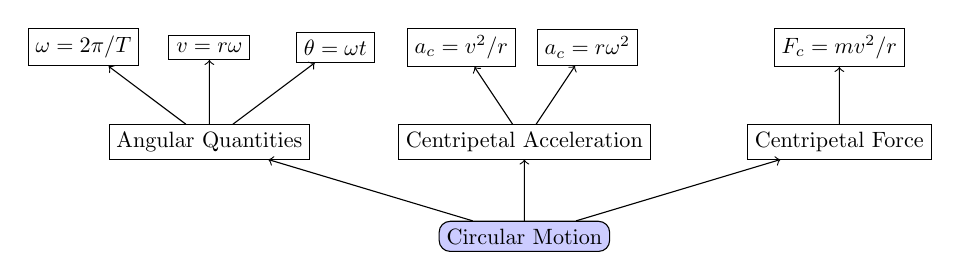
\begin{tikzpicture}[scale=0.8, transform shape]
\node[draw,rounded corners,fill=blue!20] (root) at (0,0) {Circular Motion};

% Level 1: Categories
\node[draw] (ang) at (-5,1.5) {Angular Quantities};
\node[draw] (accel) at (0,1.5) {Centripetal Acceleration};
\node[draw] (force) at (5,1.5) {Centripetal Force};

% Level 2: Equations
% Children of Angular Quantities
\node[draw] (w) at (-7,3) {$\omega = 2\pi/T$};
\node[draw] (v) at (-5,3) {$v = r\omega$};
\node[draw] (theta) at (-3,3) {$\theta = \omega t$};

% Children of Centripetal Acceleration
\node[draw] (ac1) at (-1,3) {$a_c = v^2/r$};
\node[draw] (ac2) at (1,3) {$a_c = r\omega^2$};

% Child of Centripetal Force
\node[draw] (fc) at (5,3) {$F_c = mv^2/r$};

% Arrows (Root to Level 1)
\draw[->] (root) -- (ang);
\draw[->] (root) -- (accel);
\draw[->] (root) -- (force);

% Arrows (Level 1 to Level 2)
\draw[->] (ang) -- (w);
\draw[->] (ang) -- (v);
\draw[->] (ang) -- (theta);

\draw[->] (accel) -- (ac1);
\draw[->] (accel) -- (ac2);

\draw[->] (force) -- (fc);
\end{tikzpicture}
\vfill
Link to dynamics: centripetal force is the net force causing circular motion. Link to gravitation: $F = GMm/r^2$ provides centripetal force for orbits.
\end{frame}

\end{document}